\documentclass[12pt]{article}
\usepackage{bigints}
\usepackage{graphicx}			% Use this package to include images
\usepackage{amsmath}	
\usepackage{amssymb}
\usepackage{amsfonts}
\usepackage{polynom}
\usepackage{listings}
% A library of many standard math expressions
\graphicspath{ {./Images/} }
\usepackage[margin=1in]{geometry}% Sets 1in margins. 
\newcommand{\qed}[0]{$\blacksquare$}
\usepackage{fancyhdr}			% Creates headers and footers
\usepackage{enumerate}          %These two package give custom labels to a list
\usepackage[shortlabels]{enumitem}


% Creates the header and footer. You can adjust the look and feel of these here.
\pagestyle{fancy}
\fancyhead[l]{Aditya Gupta}
\fancyhead[c]{Amath Homework \#6}
\fancyhead[r]{\today}
\fancyfoot[c]{\thepage}
\renewcommand{\headrulewidth}{0.2pt} %Creates a horizontal line underneath the header
\setlength{\headheight}{15pt} %Sets enough space for the header
\begin{document}

\begin{enumerate}
\item 
\begin{enumerate}
    \item False. Euler’s method is widely used due to its simplicity, but it is not always stable, especially for stiff differential equations. Stability depends on the time-step size; for many problems, a large time step can make Euler’s method unstable, causing solutions to diverge. Higher-order methods such as Runge-Kutta are often preferred in practice due to better stability and accuracy.
    
    \item True. Numerical errors accumulate as we step forward in time, causing the absolute error to increase for larger values of \( t \). This happens because local truncation errors at each step compound over multiple iterations. More stable methods (e.g., implicit methods or adaptive step-size control) can help mitigate this issue, but the trend remains.
\end{enumerate}

\item
\begin{enumerate}
    \item 
    
    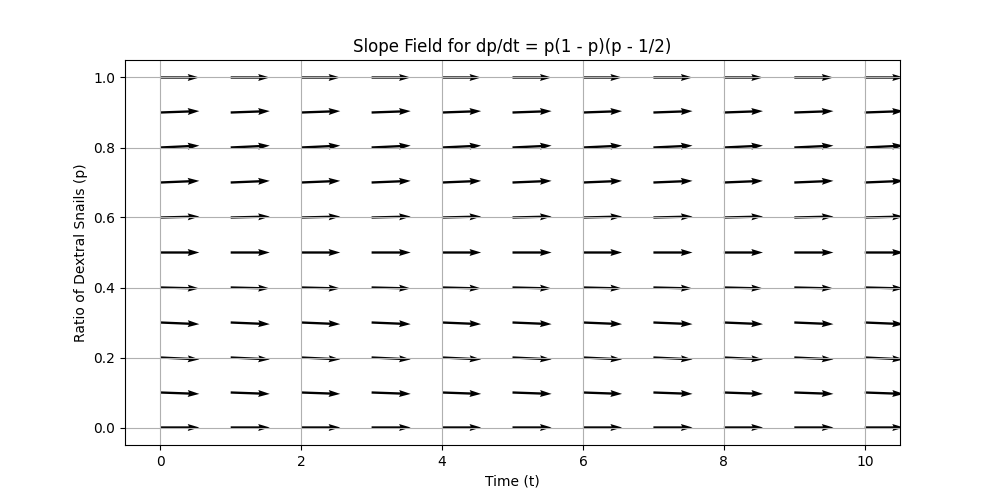
\includegraphics[width=1\linewidth]{AMath301/Figure_1.png}
    \item Interpretation of the slope field.

    The slope field helps analyze the long-term behavior of \( p(t) \) as \( t \) increases:

    \begin{itemize}
        \item If \( p(0) > 0.5 \), then \( p(t) \) increases over time and approaches \( p = 1 \), meaning dextral snails become dominant.
        \item If \( p(0) < 0.5 \), then \( p(t) \) decreases over time and approaches \( p = 0 \), meaning sinistral snails become dominant.
        \item If \( p(0) = 0.5 \), it is an unstable equilibrium. Any slight increase (e.g., \( p(0) = 0.5001 \)) will cause \( p(t) \) to move toward 1, while any slight decrease will cause \( p(t) \) to move toward 0.
    \end{itemize}

    In conclusion, the population will evolve toward one of the two extremes based on whether the initial proportion of dextral snails is above or below \( 0.5 \).
\end{enumerate}

\item 
\begin{enumerate}

    \item Consider the initial value problem:
    \[
    \frac{dy}{dt} + y^2 = 0, \quad y(0) = 1
    \]

    \item \textbf{Two iterations of Forward Euler’s Method}

    The Forward Euler's Method is given by:
    \[
    y_{n+1} = y_n + \Delta t \cdot f(t_n, y_n)
    \]
    where:
    \[
    f(t, y) = -y^2
    \]
    Given \( \Delta t = \frac{1}{4} \) and \( y(0) = 1 \), we compute the first two iterations.

    \textbf{Step 1: Compute \( y_1 \) at \( t = \frac{1}{4} \)}
    \[
    y_1 = y_0 + \Delta t \cdot f(0, y_0)
    \]
    \[
    y_1 = 1 + \frac{1}{4} \cdot (-1^2)
    \]
    \[
    y_1 = 1 - \frac{1}{4} = \frac{3}{4}
    \]

    \textbf{Step 2: Compute \( y_2 \) at \( t = \frac{1}{2} \)}
    \[
    y_2 = y_1 + \Delta t \cdot f\left(\frac{1}{4}, y_1\right)
    \]
    \[
    y_2 = \frac{3}{4} + \frac{1}{4} \cdot \left(-\left(\frac{3}{4}\right)^2\right)
    \]
    \[
    y_2 = \frac{3}{4} - \frac{1}{4} \cdot \frac{9}{16}
    \]
    \[
    y_2 = \frac{3}{4} - \frac{9}{64}
    \]
    \[
    y_2 = \frac{48}{64} - \frac{9}{64} = \frac{39}{64}
    \]

    Thus, after two iterations using Forward Euler’s Method:
    \[
    y_1 = \frac{3}{4}, \quad y_2 = \frac{39}{64}
    \]

    \item \textbf{Two iterations of Backward Euler’s Method}

    The Backward Euler's Method is given by:
    \[
    y_{n+1} = y_n + \Delta t \cdot f(t_{n+1}, y_{n+1})
    \]
    which means solving the implicit equation:
    \[
    y_{n+1} + \Delta t \cdot y_{n+1}^2 = y_n
    \]

    \textbf{Step 1: Compute \( y_1 \) at \( t = \frac{1}{4} \)}
    \[
    y_1 + \frac{1}{4} y_1^2 = 1
    \]
    Rearranging:
    \[
    y_1^2 + 4 y_1 - 4 = 0
    \]
    Solving using the quadratic formula:
    \[
    y_1 = \frac{-4 \pm \sqrt{16 + 16}}{2} = \frac{-4 \pm \sqrt{32}}{2} = \frac{-4 \pm 4\sqrt{2}}{2} = -2 \pm 2\sqrt{2}
    \]
    Since \( y > 0 \), we take:
    \[
    y_1 = -2 + 2\sqrt{2}
    \]

    \textbf{Step 2: Compute \( y_2 \) at \( t = \frac{1}{2} \)}
    \[
    y_2 + \frac{1}{4} y_2^2 = y_1
    \]
    Substituting \( y_1 = -2 + 2\sqrt{2} \):
    \[
    y_2^2 + 4 y_2 - 4(-2 + 2\sqrt{2}) = 0
    \]
    \[
    y_2^2 + 4y_2 + 8 - 8\sqrt{2} = 0
    \]

    Solving using the quadratic formula:
    \[
    y_2 = \frac{-4 \pm \sqrt{16 - 32 + 64\sqrt{2}}}{2} = \frac{-4 \pm \sqrt{48 - 64\sqrt{2}}}{2}
    \]

    Approximating, the positive root gives:
    \[
    y_2 = -2 + 2\sqrt{2 - \sqrt{2}}
    \]

    Thus, after two iterations using Backward Euler’s Method:
    \[
    y_1 = -2 + 2\sqrt{2}, \quad y_2 = -2 + 2\sqrt{2 - \sqrt{2}}
    \]

\end{enumerate}
\item 
\begin{enumerate}
    \item Convert the second-order ODE to a system of first-order equations:

    The given equation:

    \[
    \frac{d^2\theta}{dt^2} + \sin(\theta) = 0
    \]

    Define \( \omega(t) \) as the angular velocity:

    \[
    \omega = \frac{d\theta}{dt}
    \]

    Rewriting the second-order equation into a system:

    \[
    \frac{d\theta}{dt} = \omega, \quad \frac{d\omega}{dt} = -\sin(\theta)
    \]

    In vector notation, define:

    \[
    v =
    \begin{bmatrix}
    \theta \\
    \omega
    \end{bmatrix}
    \]

    Then the system becomes:

    \[
    \frac{dv}{dt} =
    \begin{bmatrix}
    \omega \\
    -\sin(\theta)
    \end{bmatrix}
    \]

    \item Write the initial condition in vector notation:

    The problem gives the initial conditions:

    \[
    \theta(0) = \frac{\pi}{6}, \quad \omega(0) = 0
    \]

    Thus, the initial vector is:

    \[
    v_0 =
    \begin{bmatrix}
    \frac{\pi}{6} \\
    0
    \end{bmatrix}
    \]

    \item Compute \( ṽ_1 \) using Euler's step:

    Heun’s method starts with a regular Euler step:

    \[
    ṽ_1 = v_0 + h f(t_0, v_0)
    \]

    Given \( h = \frac{1}{4} \), we substitute:

    \[
    f(t_0, v_0) =
    \begin{bmatrix}
    \omega_0 \\
    -\sin(\theta_0)
    \end{bmatrix}
    =
    \begin{bmatrix}
    0 \\
    -\sin\left(\frac{\pi}{6}\right)
    \end{bmatrix}
    =
    \begin{bmatrix}
    0 \\
    -\frac{1}{2}
    \end{bmatrix}
    \]

    Now, applying the Euler step:

    \[
    ṽ_1 = 
    \begin{bmatrix}
    \frac{\pi}{6} \\
    0
    \end{bmatrix}
    + \frac{1}{4}
    \begin{bmatrix}
    0 \\
    -\frac{1}{2}
    \end{bmatrix}
    \]

    \[
    =
    \begin{bmatrix}
    \frac{\pi}{6} \\
    -\frac{1}{8}
    \end{bmatrix}
    \]

    \item Compute \( v_1 \) using Heun’s correction step:

    Heun’s method uses the formula:

    \[
    v_1 = v_0 + \frac{h}{2} \left( f(t_0, v_0) + f(t_1, ṽ_1) \right)
    \]

    First, compute \( f(t_1, ṽ_1) \):

    \[
    f(t_1, ṽ_1) =
    \begin{bmatrix}
    \omegã_1 \\
    -\sin(\thetã_1)
    \end{bmatrix}
    =
    \begin{bmatrix}
    -\frac{1}{8} \\
    -\sin\left(\frac{\pi}{6}\right)
    \end{bmatrix}
    =
    \begin{bmatrix}
    -\frac{1}{8} \\
    -\frac{1}{2}
    \end{bmatrix}
    \]

    Compute the average of the slopes:

    \[
    \frac{1}{2} \left( f(t_0, v_0) + f(t_1, ṽ_1) \right)
    \]

    \[
    =
    \frac{1}{2} \left( 
    \begin{bmatrix}
    0 \\
    -\frac{1}{2}
    \end{bmatrix}
    + 
    \begin{bmatrix}
    -\frac{1}{8} \\
    -\frac{1}{2}
    \end{bmatrix}
    \right)
    \]

    \[
    =
    \frac{1}{2}
    \begin{bmatrix}
    -\frac{1}{8} \\
    -1
    \end{bmatrix}
    =
    \begin{bmatrix}
    -\frac{1}{16} \\
    -\frac{1}{2}
    \end{bmatrix}
    \]

    Finally, applying the correction step:

    \[
    v_1 = 
    \begin{bmatrix}
    \frac{\pi}{6} \\
    0
    \end{bmatrix}
    + \frac{1}{4}
    \begin{bmatrix}
    -\frac{1}{16} \\
    -\frac{1}{2}
    \end{bmatrix}
    \]

    \[
    =
    \begin{bmatrix}
    \frac{\pi}{6} - \frac{1}{64} \\
    -\frac{1}{8}
    \end{bmatrix}
    \]

\end{enumerate}


\end{enumerate}

\end{document}
